\begin{block}{Implementation}
\begin{columns}
\begin{column}{.65\textwidth}
    Full simulation study at $\sqrt{s} = 250~\GeV$ \\
    (MC2020 ILD mass production).
    \begin{itemize}
        \item $\sqrt{s} = 250~\GeV$ ideal for the Higgsstrahlung process.
        \item Considered backgrounds: Standard Model (SM) processes
            with 2 or 4 fermions in the final state.
        \item $\geq 400$k simulated events/SM Higgs decay mode.
        \item Polarized initial beams: 80\% left (30\% right) polarized electron (positron) beam.
        \item 2000~fb$^{-1}$ integrated luminosity.
    \end{itemize}
\end{column}
\begin{column}{.35\textwidth}
    \begin{figure}
        \centering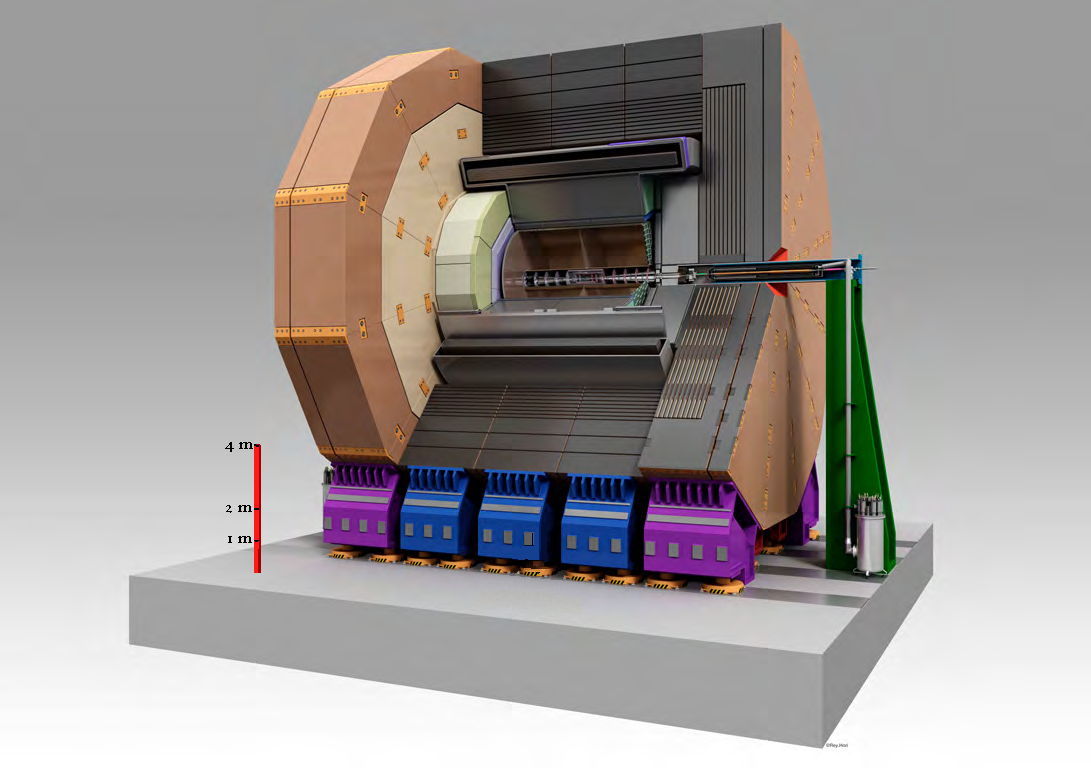
\includegraphics[width=\textwidth]{IGP_ILD}
    \end{figure}
\end{column}
\end{columns}
\end{block}
